\chapter{Mediciones}\label{cap:mediciones}
El montaje de la \cref{fig:montaje} usa los valores $R=\SI{47}{\ohm}$, $L=\SI{10}{\milli\henry}$ y
$C=\SI{100}{\nano\farad}$.\index{montaje experimental}

\begin{figure}[htbp]
  \centering
  \begin{subfigure}[b]{0.48\textwidth}
    \centering
    \begin{circuitikz}[scale=0.85, transform shape]
      \draw (0,0) to[sV, l=$v_s(t)$] (0,3)
            to[R, l=$R$, -*] (3,3)
            to[L, l=$L$] (5,3)
            to[C, l=$C$, v^>=$v_C$] (5,0) -- (0,0);
    \end{circuitikz}
    \caption{Esquema.}\label{fig:esquema}
  \end{subfigure}\hfill
  \begin{subfigure}[b]{0.48\textwidth}
    \centering
    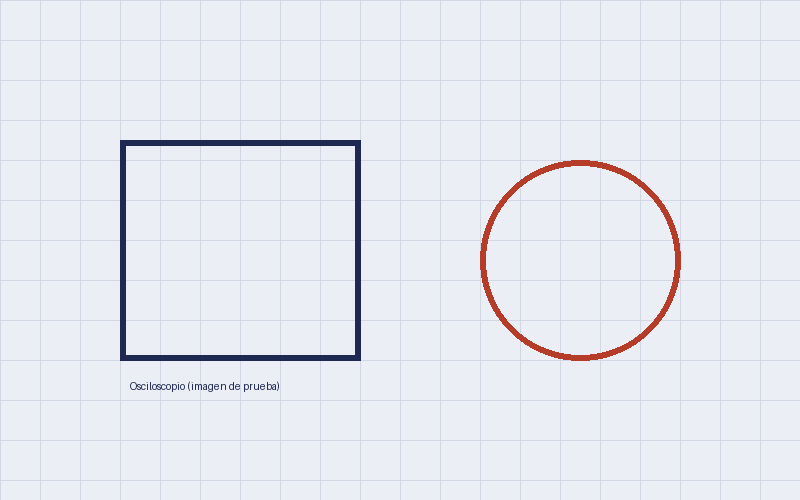
\includegraphics[width=\linewidth]{figuras/foto del laboratorio.png}
    \caption{Montaje real.}\label{fig:foto}
  \end{subfigure}
  \caption{Circuito \gls{rlc} serie usado en las mediciones.}\label{fig:montaje}
\end{figure}

\begin{figure}[htbp]
  \centering
  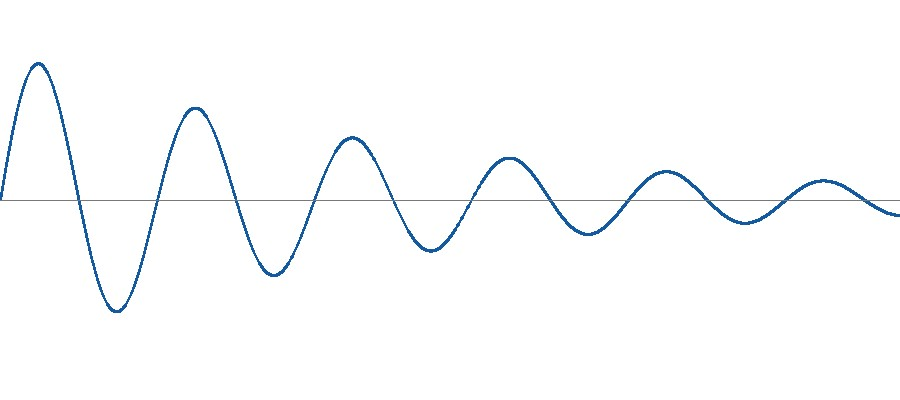
\includegraphics[width=0.8\textwidth]{figuras/señal medida.jpg}
  \caption{Señal medida en el osciloscopio (nombre de archivo con tilde y espacio).}\label{fig:senal}
\end{figure}

\section{Tabla de mediciones}
La \cref{tab:mediciones} es larga a propósito: cruza de página y repite su encabezado.

\begin{longtable}{
  S[table-format=6.0]
  S[table-format=2.3]
  S[table-format=2.3]
  S[table-format=+3.1]
  c}
  \caption{Respuesta en frecuencia medida.}\label{tab:mediciones}\\
  \toprule
  {$f$ (\si{\hertz})} & {$V_\text{in}$ (\si{\volt})} & {$V_C$ (\si{\volt})} & {$\varphi$ (\si{\degree})} & {Nota}\\
  \midrule
  \endfirsthead
  \multicolumn{5}{l}{\small\itshape (continuación de la \cref{tab:mediciones})}\\
  \toprule
  {$f$ (\si{\hertz})} & {$V_\text{in}$ (\si{\volt})} & {$V_C$ (\si{\volt})} & {$\varphi$ (\si{\degree})} & {Nota}\\
  \midrule
  \endhead
  \midrule\multicolumn{5}{r}{\small\itshape sigue en la página siguiente}\\
  \endfoot
  \bottomrule
  \endlastfoot
  100 & 2.000 & 2.001 & -0.2 & \\
  112 & 2.000 & 2.001 & -0.2 & \\
  125 & 2.000 & 2.001 & -0.2 & \\
  140 & 2.000 & 2.002 & -0.2 & \\
  156 & 2.000 & 2.002 & -0.3 & \\
  174 & 2.000 & 2.002 & -0.3 & \\
  194 & 2.000 & 2.003 & -0.3 & \\
  217 & 2.000 & 2.004 & -0.4 & \\
  243 & 2.000 & 2.005 & -0.4 & \\
  272 & 2.000 & 2.006 & -0.5 & \\
  304 & 2.000 & 2.007 & -0.5 & \\
  340 & 2.000 & 2.009 & -0.6 & \\
  380 & 2.000 & 2.011 & -0.6 & \\
  425 & 2.000 & 2.014 & -0.7 & \\
  476 & 2.000 & 2.018 & -0.8 & \\
  533 & 2.000 & 2.022 & -0.9 & \\
  596 & 2.000 & 2.028 & -1.0 & \\
  667 & 2.000 & 2.035 & -1.1 & \\
  747 & 2.000 & 2.045 & -1.3 & \\
  836 & 2.000 & 2.056 & -1.5 & \\
  936 & 2.000 & 2.071 & -1.6 & \\
  1048 & 2.000 & 2.090 & -1.9 & \\
  1173 & 2.000 & 2.113 & -2.1 & \\
  1313 & 2.000 & 2.144 & -2.4 & \\
  1470 & 2.000 & 2.184 & -2.7 & \\
  1646 & 2.000 & 2.236 & -3.1 & \\
  1843 & 2.000 & 2.305 & -3.6 & \\
  2064 & 2.000 & 2.398 & -4.2 & \\
  2311 & 2.000 & 2.525 & -4.9 & \\
  2588 & 2.000 & 2.704 & -5.9 & \\
  2898 & 2.000 & 2.968 & -7.3 & \\
  3245 & 2.000 & 3.378 & -9.3 & \\
  3634 & 2.000 & 4.077 & -12.6 & \\
  4070 & 2.000 & 5.460 & -19.2 & \\
  4170 & 2.000 & 5.938 & -21.4 & \\
  4270 & 2.000 & 6.509 & -24.2 & \\
  4370 & 2.000 & 7.198 & -27.7 & \\
  4470 & 2.000 & 8.031 & -32.0 & \\
  4570 & 2.000 & 9.034 & -37.6 & \\
  4670 & 2.000 & 10.213 & -44.8 & \\
  4770 & 2.000 & 11.510 & -54.2 & \\
  4870 & 2.000 & 12.715 & -66.1 & \\
  4970 & 2.000 & 13.436 & -80.4 & \\
  5070 & 2.000 & 13.293 & -95.6 & \\
  5170 & 2.000 & 12.319 & -109.9 & \\
  5270 & 2.000 & 10.924 & -121.8 & \\
  5370 & 2.000 & 9.501 & -131.1 & \\
  5470 & 2.000 & 8.238 & -138.3 & \\
  5570 & 2.000 & 7.180 & -143.8 & \\
  5670 & 2.000 & 6.309 & -148.1 & \\
  5770 & 2.000 & 5.593 & -151.5 & \\
  5870 & 2.000 & 5.002 & -154.3 & \\
  5970 & 2.000 & 4.509 & -156.6 & \\
  6070 & 2.000 & 4.093 & -158.5 & \\
  6798 & 2.000 & 2.357 & -166.3 & \\
  7613 & 2.000 & 1.530 & -170.1 & \\
  8526 & 2.000 & 1.060 & -172.3 & \\
  9549 & 2.000 & 0.765 & -173.8 & \\
  10694 & 2.000 & 0.567 & -174.9 & \\
  11977 & 2.000 & 0.428 & -175.7 & \\
  13414 & 2.000 & 0.327 & -176.3 & \\
  15023 & 2.000 & 0.252 & -176.8 & \\
  16825 & 2.000 & 0.196 & -177.2 & \\
  18844 & 2.000 & 0.153 & -177.6 & \\
  21105 & 2.000 & 0.121 & -177.8 & \\
  23637 & 2.000 & 0.095 & -178.1 & \\
  26473 & 2.000 & 0.075 & -178.3 & \\
  29649 & 2.000 & 0.059 & -178.5 & \\
  33206 & 2.000 & 0.047 & -178.7 & \\
  37190 & 2.000 & 0.037 & -178.8 & \\
  41652 & 2.000 & 0.030 & -179.0 & \\
  46650 & 2.000 & 0.024 & -179.1 & \\
  52248 & 2.000 & 0.019 & -179.2 & \\
  58517 & 2.000 & 0.015 & -179.3 & \\
  65539 & 2.000 & 0.012 & -179.3 & \\
  73403 & 2.000 & 0.009 & -179.4 & \\
  82211 & 2.000 & 0.008 & -179.5 & \\
  92076 & 2.000 & 0.006 & -179.5 & \\
  103125 & 2.000 & 0.005 & -179.6 & \\
  115500 & 2.000 & 0.004 & -179.6 & \\
  129360 & 2.000 & 0.003 & -179.7 & \\
  144883 & 2.000 & 0.002 & -179.7 & \\
  162268 & 2.000 & 0.002 & -179.7 & \\
  181740 & 2.000 & 0.002 & -179.8 & \\
\end{longtable}

\section{Resumen con notas al pie en la tabla}
\begin{table}[htbp]
  \centering
  \begin{threeparttable}
    \caption{Comparación teórica y medida.}\label{tab:resumen}
    \rowcolors{2}{gray!10}{white}
    \begin{tabular}{l S[table-format=4.1] S[table-format=4.1] S[table-format=1.2]}
      \toprule
      Magnitud & {Teórico} & {Medido} & {Error (\si{\percent})}\\
      \midrule
      $f_0$ (\si{\hertz})\tnote{a} & 5032.9 & 5010.0 & 0.45\\
      $Q$\tnote{b} & 6.7 & 6.4 & 4.48\\
      \multirow{2}{*}{Ancho de banda (\si{\hertz})} & 751.0 & 782.0 & 4.13\\
       & 751.0 & 779.5 & 3.79\\
      \bottomrule
    \end{tabular}
    \begin{tablenotes}\footnotesize
      \item[a] Con la \cref{eq:resonancia}.
      \item[b] $Q=f_0/\Delta f$.
    \end{tablenotes}
  \end{threeparttable}
\end{table}
